\section{Implementation paths and controlled training studies}
\label{sec:C08:implementation}
The inspected TRL snapshot contains \texttt{DPOTrainer} in \path{trl/trainer/dpo_trainer.py}, with reference-log-probability preparation and loss computation, and \texttt{GRPOTrainer} in \path{trl/trainer/grpo_trainer.py}, with reward collection and per-token log-probability routines~\cite{rewrite_trl_repo}. These code locations identify a concrete implementation surface; they do not establish that every option matches the original papers. Record the selected loss type, reward normalization, reference policy, sampling backend, masking, clipping, and synchronization behavior. A repository version without configuration is not a reproducible algorithm.

The reductions are visible in \path{GRPOTrainer._compute_loss}. For a local batch of $B$ completions with binary action mask $m_{bt}$, per-token surrogate contribution $\ell_{bt}$, positive counts $n_b=\sum_tm_{bt}$, and configured maximum length $T_{\max}$, three inspected branches reduce as
\begin{equation}
\begin{aligned}
 L_{\mathrm{grpo}}&=\frac1B\sum_b\frac{\sum_tm_{bt}\ell_{bt}}{n_b},\\
 L_{\mathrm{bnpo}}&=\frac{\sum_{b,t}m_{bt}\ell_{bt}}{\sum_bn_b},\\
 L_{\mathrm{dr}}&=\frac{\sum_{b,t}m_{bt}\ell_{bt}}{BT_{\max}}.
\end{aligned}
\end{equation}
These equations describe the positive-count case before the branch's accumulation scaling; the code clamps empty denominators and other loss types use different window-level normalization~\cite{rewrite_trl_repo}. They demonstrate why the class name does not identify the objective. Varying completion length changes relative weights even with the same sampled rewards and token ratios.

For preference learning, \path{DPOTrainer.compute_ref_log_probs} and \path{_compute_loss} both construct completion masks and distinguish cached reference scores from a live reference forward. In the standard summed-log-probability branch, changing to a length-normalized variant is an explicit loss change. Cached reference scores should therefore be bound to the reference or adapter identity, tokenizer, serialization and exact completion mask; the cache's existence alone does not validate their compatibility with a later batch. This is a proposed integrity check on an inspected dataflow, not an executed trainer comparison.


Let $z_k=(\theta_k,\omega_k)$ be the policy and optimizer state at update $k$, and fix reference parameters $\bar\theta=\theta_0$. The manifest $\nu_k$ records the environment, context construction, sampling, and execution versions. For positive integer batch size $b_k$ and batch $X_k=(x_{ki})_{i=1}^{b_k}$, isolated trajectories satisfy
\begin{equation}
\label{eq:C08:mathematical-rollout}
\begin{aligned}
 \bar\theta_k&=\bar\theta,\\
 \boldsymbol\tau_k\mid X_k,\nu_k
 &\sim\bigotimes_{i=1}^{b_k}
       P_{\theta_k,\nu_k}(\,\cdot\mid x_{ki}),\\
 r_{ki}&=V_\varphi\!\left(\mathcal O(\tau_{ki}),x_{ki}\right),\\
 \boldsymbol A_k&=\mathcal G(\boldsymbol r_k,\boldsymbol\tau_k).
\end{aligned}
\end{equation}
Here $\mathcal O$ extracts recorded environment outcomes, $V_\varphi$ is the separately specified outcome scorer, and $\mathcal G$ is the declared advantage estimator. The product law assumes independent initialization and randomization of isolated rollout environments; shared mutable state instead requires a joint trajectory law. Independence from the actor's update does not make the scorer an error-free oracle.

For trajectory $i$ at trained model decision $t\in\mathcal I(\tau_{ki})$, let $c^{\mathrm b}_{kit}$ be the actual behavior input and $\widetilde c_{kit}$ the input used to recompute its probability during training. Let $\nu^{\mathrm b}_{kit}$ and $\widetilde\nu_{kit}$ record the corresponding serialization and forward-computation contracts, apart from explicitly designated behavior and target parameter values. The admissibility indicator is
\begin{equation}
\label{eq:C08:conditioning-gate}
 I_k=\mathbf1\!\left\{
 \begin{aligned}
 &\widetilde c_{kit}=c^{\mathrm b}_{kit},\\
 &\widetilde\nu_{kit}=\nu^{\mathrm b}_{kit}
 \quad\forall i,\ t\in\mathcal I(\tau_{ki})
 \end{aligned}\right\}.
\end{equation}
Intentional off-policy updates need the declared behavior-probability correction rather than an assertion that policy versions are equal. The equality above concerns the inputs and forward semantics used to evaluate the required probabilities. It does not replace the earlier zero-update logit test.

On an admissible batch, a chosen policy-loss functional $\mathcal L$ and optimizer $\mathcal U_k$ give
\begin{equation}
\label{eq:C08:mathematical-update}
\begin{aligned}
 g_k&=\left.\nabla_\theta
 \mathcal L(\theta;\boldsymbol\tau_k,\boldsymbol A_k,\bar\theta)
 \right|_{\theta=\theta_k},\\
 z_{k+1}&=\mathcal U_k(z_k,g_k),\qquad I_k=1,\\
 \boldsymbol e_{k+1}
 &=\mathcal E(\theta_{k+1};D_{\mathrm a},\nu_{\mathrm a}).
\end{aligned}
\end{equation}
The sampled trajectories, rewards, and estimated advantages are held fixed in this derivative; it is the gradient of the chosen empirical surrogate, not an assertion about an unbiased total derivative through trajectory sampling. Normalization, clipping, and synchronization are part of the specified loss and optimizer. When $I_k=0$, this update is not admissible until the conditioning discrepancy is resolved or a justified alternative estimator is supplied. The evaluator $\mathcal E$ uses a separate audit population $D_{\mathrm a}$ and manifest $\nu_{\mathrm a}$. Its outputs are report-only for this protocol; feeding them into training or hyperparameter selection converts the audit into selection feedback and requires a separate confirmatory evaluation. These equations organize the implementation contract rather than identify a universal post-training objective.

A fair study includes supervised fine-tuning, an offline preference method, and online reinforcement learning where feasible, with matched initial checkpoints and clearly separated data budgets. Report both environment interactions and generated tokens. An online method's access to additional trajectories is an important advantage, not an incidental detail. Include a no-learning inference baseline that spends comparable compute on independent sampling and verification. Otherwise training gains can be confused with the benefit of simply allocating more attempts at evaluation time.

{\small\setlength{\tabcolsep}{3pt}
\begin{table}[!htbp]
\centering
\caption{Mechanistic ablations for agent post-training.}\label{tab:C08:ablations}
\begin{tabular}{L{29mm}L{37mm}L{40mm}}

\toprule Ablation & Preserved controls & Diagnostic measurement\\\midrule
No outcome verifier & Same generated trajectories & Reward exploitation and false acceptance.\\
No context editing & Same policy and tasks & Conditioning mismatch contribution.\\
Fixed versus adaptive memory & Same storage budget & Credit assignment to memory actions.\\
Group size change & Same total generation budget & Contrast and estimator variance.\\
Reference strength change & Same preference data & Drift, support, and capability retention.\\
\bottomrule
\end{tabular}
\end{table}
}

\subsection{Harness-native reinforcement learning and segmented behavior policies}
\label{sec:C08:harnessnative}
OpenForgeRL's current third version captures the deployment harness's actual model requests through an inference proxy and executes rollouts in remote containerized environments. Its Section 3 redistributes terminal reward to captured request-response samples, uses wall-clock timeouts across harnesses with incompatible turn definitions, and discards trajectories ending in infrastructure errors or timeout~\cite{rewrite_openforge2026}. The intervention preserves the deployed context constructor and control flow during training rather than substituting a simpler chat loop. It does not by itself guarantee correct token alignment or unbiased treatment of discarded episodes.

Molt's third version supplies complementary contracts. Sections 4.2--4.5 record sampled token identifiers, action ranges, behavior probabilities, and multimodal inputs; a rewritten conversation prefix starts a new segment while preserving the rollout identity. Partial generation across weight refits requires probability correction, and expert-routing replay is distinct from freezing an MoE router~\cite{rewrite_molt2026}. These are separate consistency conditions: using the same harness preserves the interaction procedure; exact token records preserve sampled actions; matching forward semantics preserves what their probabilities mean.

Let $c_i$ be the actual rendered context for trained action token $x_i$, and let $\mu_i(x_i\mid c_i)$ be its recorded behavior probability, potentially from a different weight version at each token. Under identical fixed harness and environment kernels, and absolute continuity of the target policy relative to behavior, the full trajectory likelihood ratio is
\begin{equation}
 W(\tau)=\prod_{i\in\mathcal I(\tau)}
 \frac{p_\theta(x_i\mid c_i)}{\mu_i(x_i\mid c_i)},
\end{equation}
where $\mathcal I(\tau)$ indexes all relevant policy-generated tokens and the nonpolicy transition factors cancel. This identity does not imply that the product is a practical low-variance estimator. Per-token clipping or rejection chooses a different bias--variance tradeoff. Reconstructing $c_i$ from a final transcript after compaction instead changes the conditional probabilities themselves and cannot be repaired by a ratio computed on that altered history.

Discarding interrupted rollouts also changes the measured population. For bounded episode return $R$ and retention indicator $D$, with $\Pr(D=1)>0$,
\begin{equation}
 \mathbb E[R\mid D=1]-\mathbb E[R]
 =\frac{\operatorname{Cov}(R,D)}{\Pr(D=1)}.
\end{equation}
Even a policy-independent network fault can correlate with task duration, and duration can correlate with difficulty. Therefore absence of a direct reward-based filter does not establish zero selection bias. Compare the native harness with a simplified training harness while holding weights, tasks, tools, sampling, and compute fixed; separately audit retained versus interrupted tasks by duration and domain. Keep tool observations out of action loss, verify segmentation after an actual prefix rewrite, and compare zero-update recomputed probabilities with the recorded behavior path before interpreting learning gains.


Figure~\ref{fig:C08:behavior-segments} isolates the mechanism and its stated information boundaries.
\begin{figure}[!htbp]
\centering
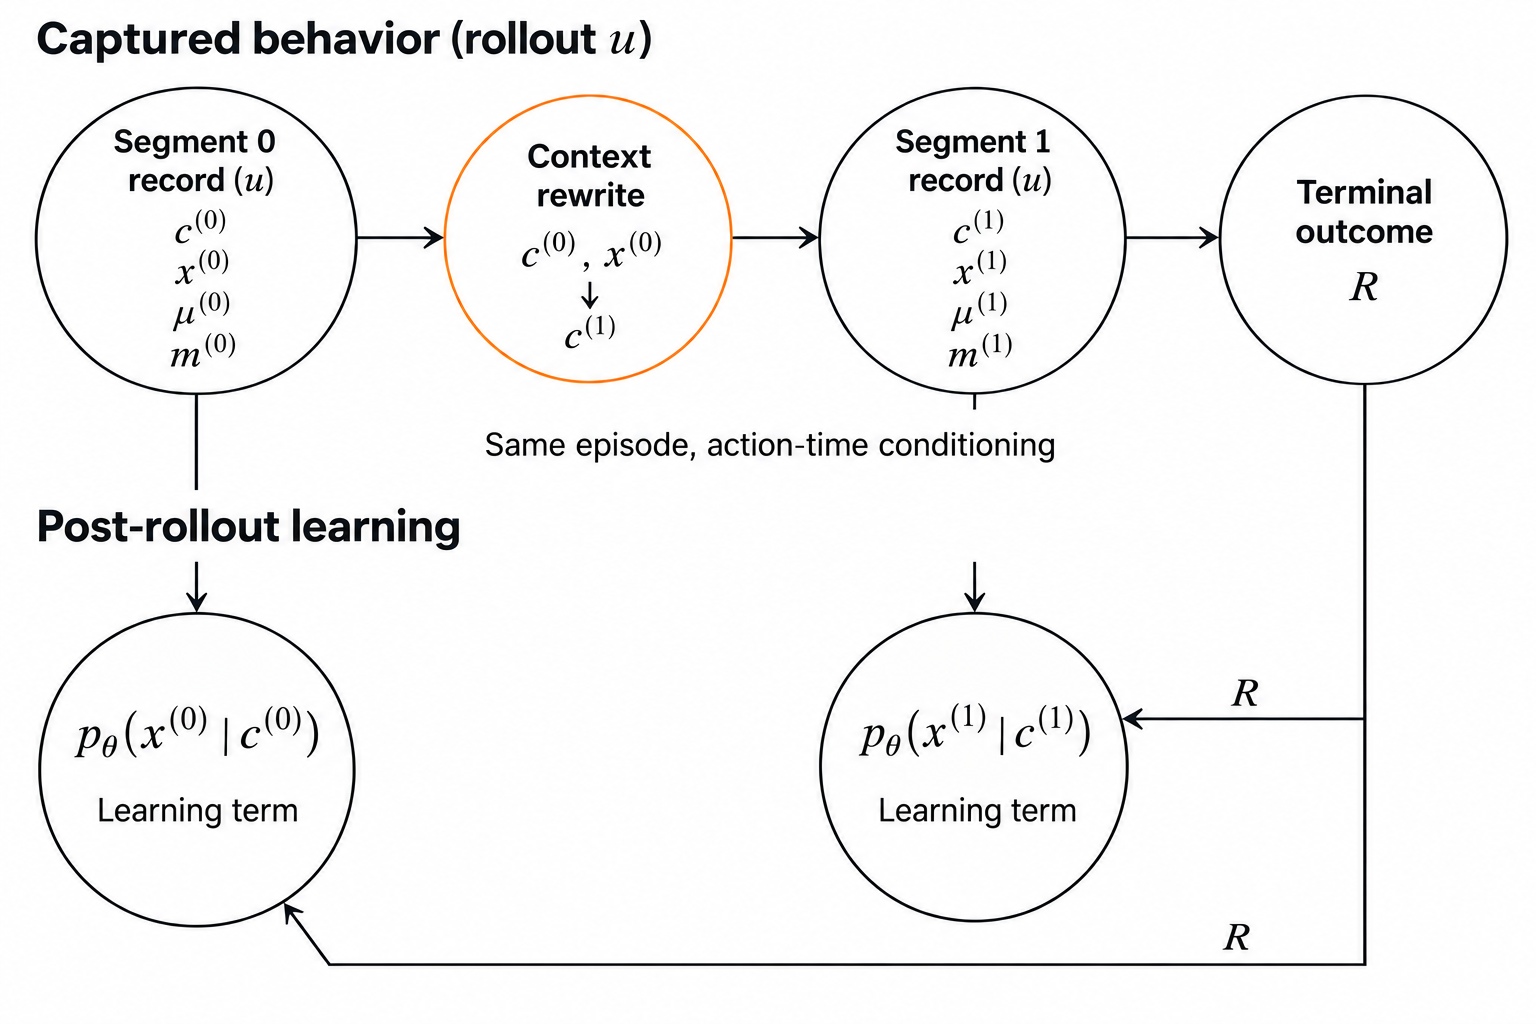
\includegraphics[width=\linewidth]{book/figures/assets/F08review.png}
\caption{A single rollout $u$ can contain multiple action-time contexts. Each segment retains context $c^{(i)}$, sampled tokens $x^{(i)}$, behavior probabilities $\mu^{(i)}$ and learning mask $m^{(i)}$. Terminal outcome $R$ may weight later learning terms; it is not an additional conditioning argument of the displayed action likelihood. The lower circles denote learning computations, not behavior calls. This schematic omits the full post-training objective and correction factors.}
\label{fig:C08:behavior-segments}
\end{figure}
